\documentclass{beamer}

\setlength{\paperwidth}{40in} % Poster width
\setlength{\paperheight}{32in} % Poster height
\newlength{\onecolwid}
\setlength{\onecolwid}{0.36\paperwidth} % Divide 1 by number of columns

\usepackage[scale=1.35]{beamerposter}
\mode<presentation>{\usetheme{isc}}
\hypersetup{pdfpagemode=UseNone,pdfstartview=FitH}
\usepackage{graphicx}
\DeclareGraphicsExtensions{.pdf,.jpg,.jpeg,.png}
\graphicspath{{figures/}}
\usepackage{amsmath}

\title{Overly Complicated and Fancy \\ Title of Poster}
\student{Joe~Miner, \textit{ECE}}
\advisor{Dr.~Joe~Miner, \textit{ECE} and \\[0.2em] Dr.~John~Miner, \textit{CS}}
\date{November XX, 20XX}

\begin{document}
\begin{frame}
\begin{columns}[t]

\begin{column}{\onecolwid}
  \begin{block}{Project Objectives}
  	\textbf{
      \begin{itemize}
		  \item Doing research
		  \item And more research
	  \end{itemize}
    }
  \end{block}

  \begin{block}{Background}
    \begin{itemize}
      \item \alert{Some important} background.
      \item See this figure:
    \end{itemize}
    \begin{figure}
      \centering
      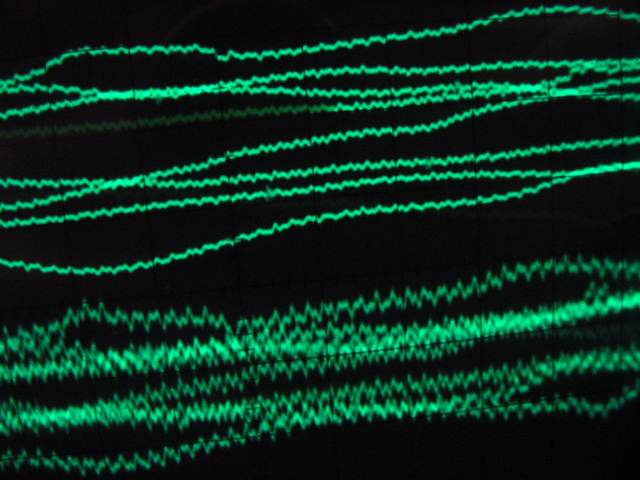
\includegraphics[width=0.60\linewidth]{sample}
      \caption{A free image from www.freeimages.com}
      \label{fig:sample}
    \end{figure}
  \end{block}

  \begin{block}{Approach}
    Work hard, play hard!

    Work hard, play hard!

    Work hard, play hard!

    And this is how:

    \begin{equation*}
      \theta = \alpha + \beta
      \label{eqn:equation}
    \end{equation*}
  \end{block}
\end{column}

\begin{column}{\onecolwid}
  \begin{block}{Results}
    Want to see some interesting results? Here you go:

    \begin{figure}
      \centering
      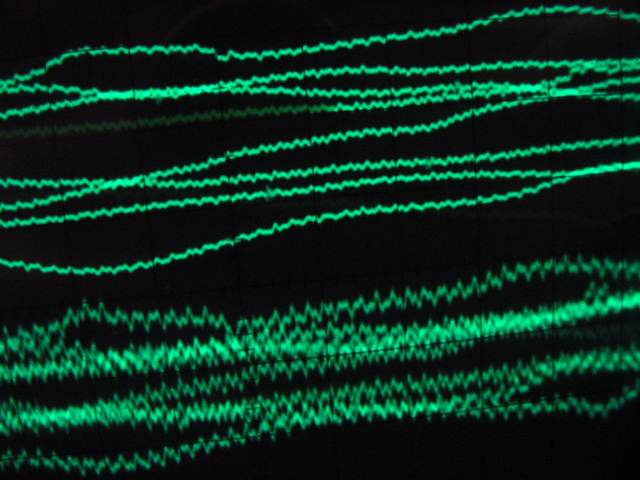
\includegraphics[width=0.80\linewidth]{sample}
      \caption{Is it a duplicate?}
      \label{fig:sample2}
    \end{figure}
  \end{block}
\end{column}

\begin{column}{\onecolwid}
  \begin{block}{Discussion}
    \begin{itemize}
      \item We are awesome
      \item Really awesome
    \end{itemize}

    \begin{table}
      \label{tab:random}
      \caption{Random numbers}
      \centering
      \begin{tabular}{c|c}
        Index         & Value \\ \hline
        $\sigma_1$    & 0.68 \\
        $\sigma_2$    & 0.42 \\
        $\sigma_3$    & 0.04
      \end{tabular}
    \end{table}
  \end{block}

  \begin{block}{Conclusions and Future Work}
    \begin{itemize}
      \item Conclusion 1
      \item Conclusion 2
    \end{itemize}
  \end{block}

  \begin{smallblock}{Acknowledgements}
    Thank you \LaTeX
  \end{smallblock}
\end{column}

\end{columns}
\end{frame}
\end{document} 